\documentclass[paper=a4,parskip=half,headings=normal]{scrreprt}
\usepackage[utf8]{inputenc} 
\usepackage[T1]{fontenc} 
\usepackage[english]{babel} 

\usepackage{graphicx}
\usepackage{float}
\usepackage[caption = false]{subfig}

%%--------------------------------------

\begin{document}
\begin{figure}

\subfloat[]{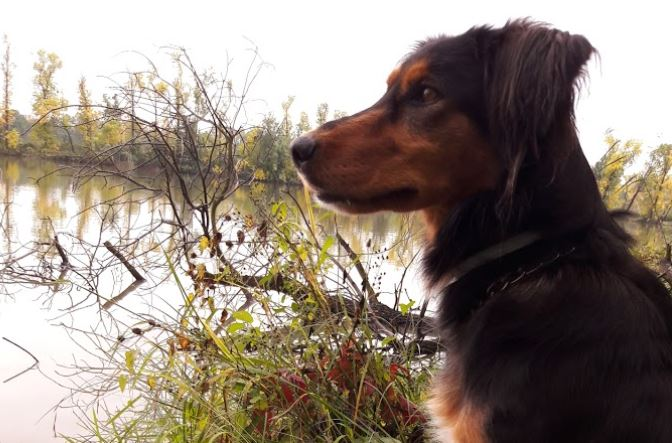
\includegraphics[width = 0.3\textwidth]{"O:/latex kurz/automate_figures/figures/daisy (1).JPG"}}
\subfloat[]{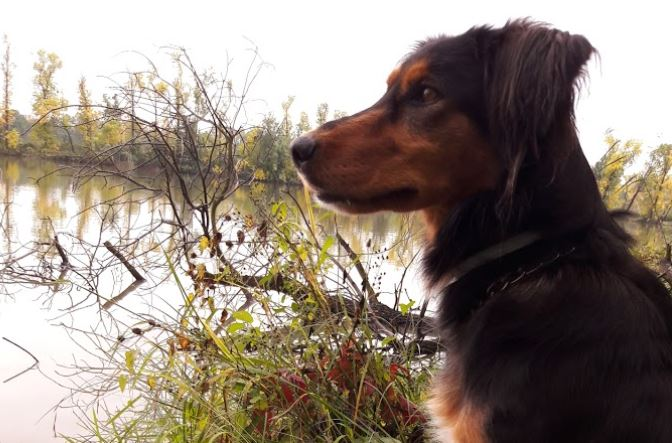
\includegraphics[width = 0.3\textwidth]{"O:/latex kurz/automate_figures/figures/daisy (10).JPG"}}
\subfloat[]{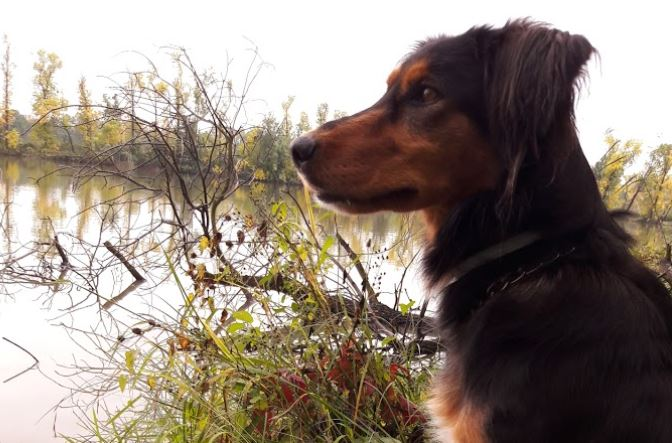
\includegraphics[width = 0.3\textwidth]{"O:/latex kurz/automate_figures/figures/daisy (11).JPG"}}\\
\subfloat[]{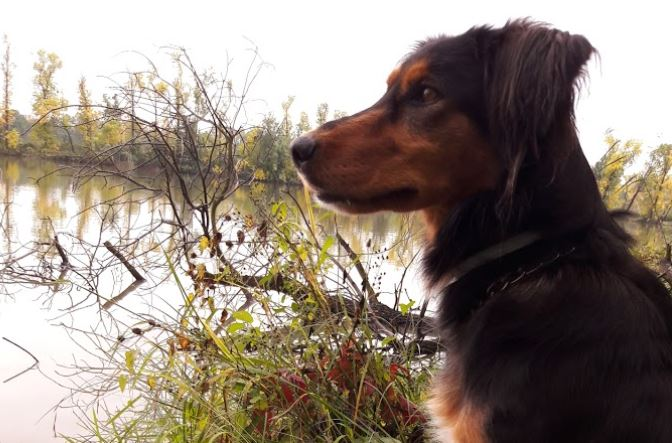
\includegraphics[width = 0.3\textwidth]{"O:/latex kurz/automate_figures/figures/daisy (12).JPG"}}
\subfloat[]{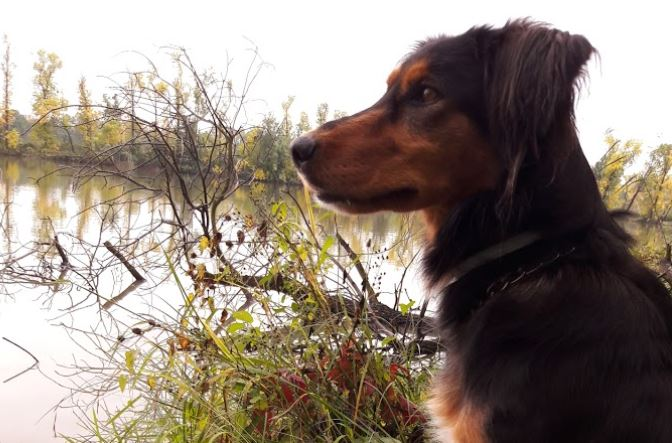
\includegraphics[width = 0.3\textwidth]{"O:/latex kurz/automate_figures/figures/daisy (13).JPG"}}
\subfloat[]{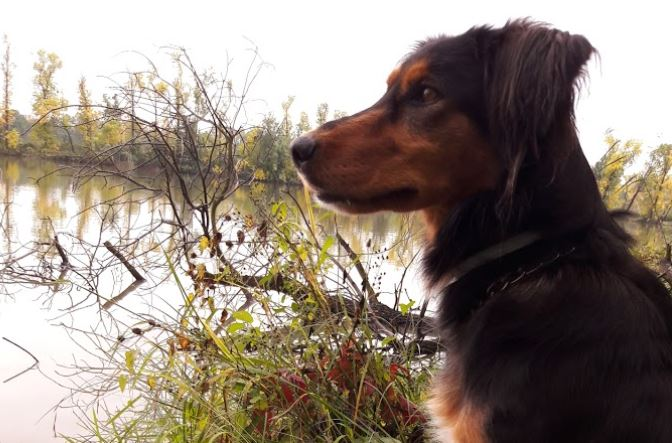
\includegraphics[width = 0.3\textwidth]{"O:/latex kurz/automate_figures/figures/daisy (14).JPG"}}\\
\subfloat[]{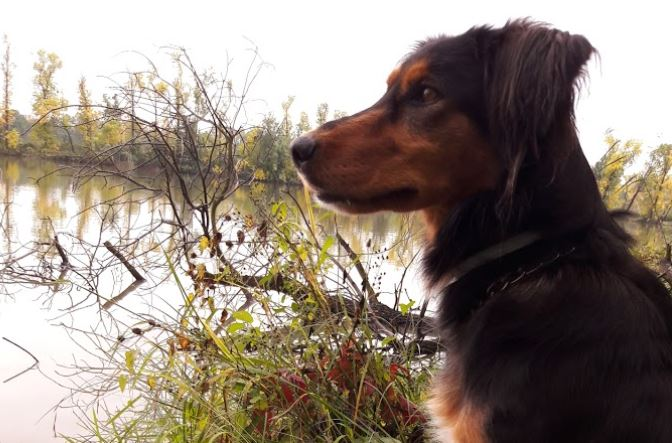
\includegraphics[width = 0.3\textwidth]{"O:/latex kurz/automate_figures/figures/daisy (15).JPG"}}
\subfloat[]{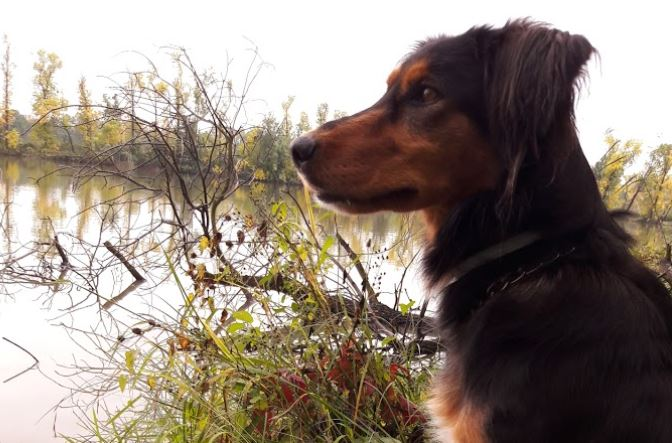
\includegraphics[width = 0.3\textwidth]{"O:/latex kurz/automate_figures/figures/daisy (16).JPG"}}
\subfloat[]{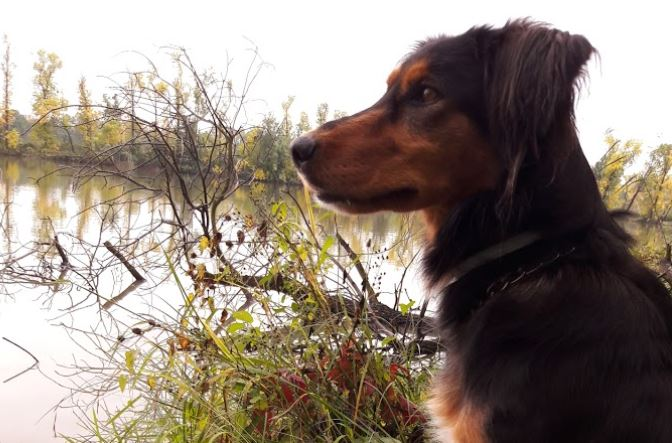
\includegraphics[width = 0.3\textwidth]{"O:/latex kurz/automate_figures/figures/daisy (17).JPG"}}\\
\subfloat[]{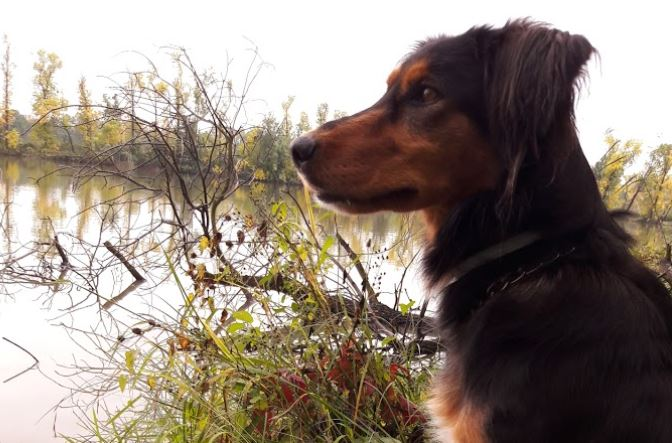
\includegraphics[width = 0.3\textwidth]{"O:/latex kurz/automate_figures/figures/daisy (18).JPG"}}
\subfloat[]{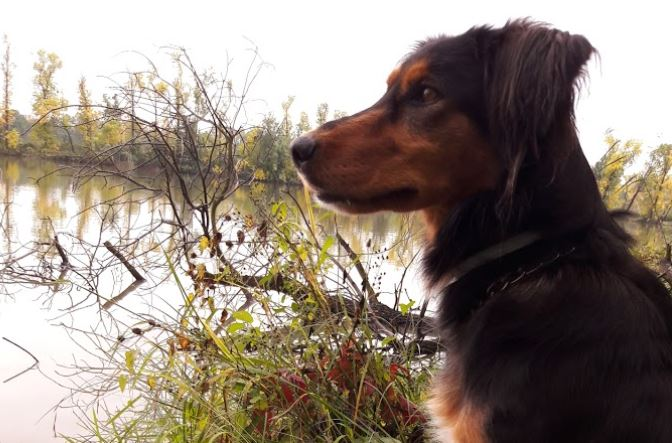
\includegraphics[width = 0.3\textwidth]{"O:/latex kurz/automate_figures/figures/daisy (19).JPG"}}
\subfloat[]{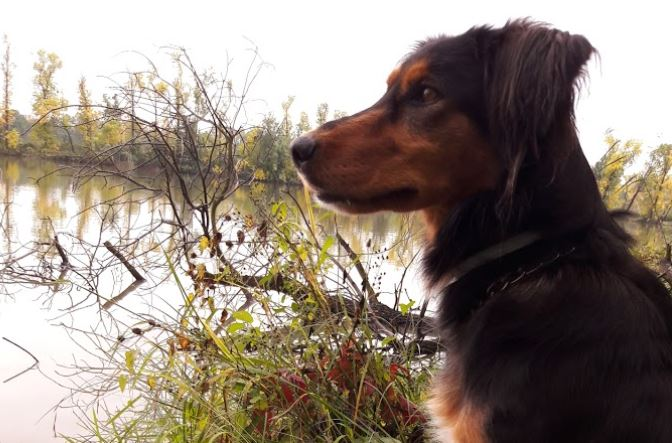
\includegraphics[width = 0.3\textwidth]{"O:/latex kurz/automate_figures/figures/daisy (2).JPG"}}\\
\caption{Caption for the figures.}
  \label{supp-fig-1}
  \end{figure}
  
  \begin{figure}

\subfloat[]{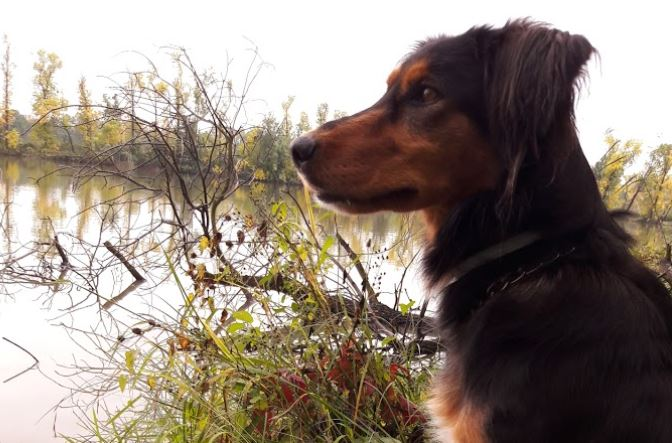
\includegraphics[width = 0.3\textwidth]{"O:/latex kurz/automate_figures/figures/daisy (20).JPG"}}
\subfloat[]{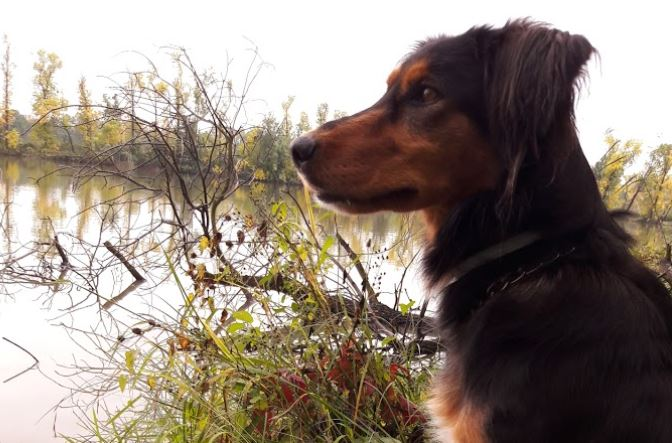
\includegraphics[width = 0.3\textwidth]{"O:/latex kurz/automate_figures/figures/daisy (21).JPG"}}
\subfloat[]{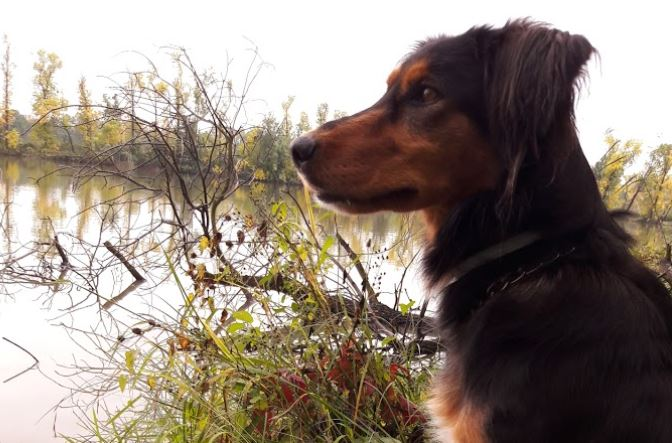
\includegraphics[width = 0.3\textwidth]{"O:/latex kurz/automate_figures/figures/daisy (22).JPG"}}\\
\subfloat[]{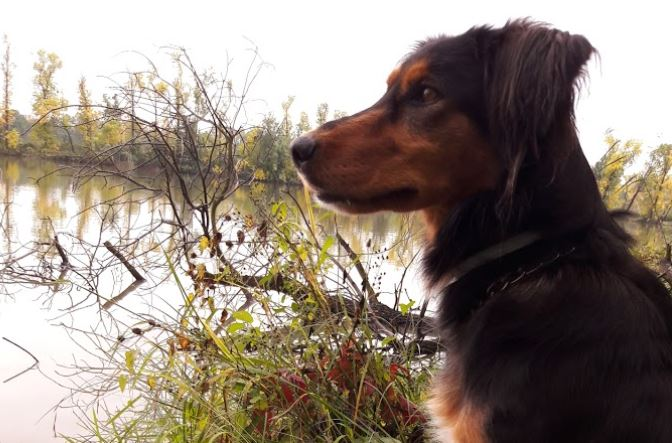
\includegraphics[width = 0.3\textwidth]{"O:/latex kurz/automate_figures/figures/daisy (23).JPG"}}
\subfloat[]{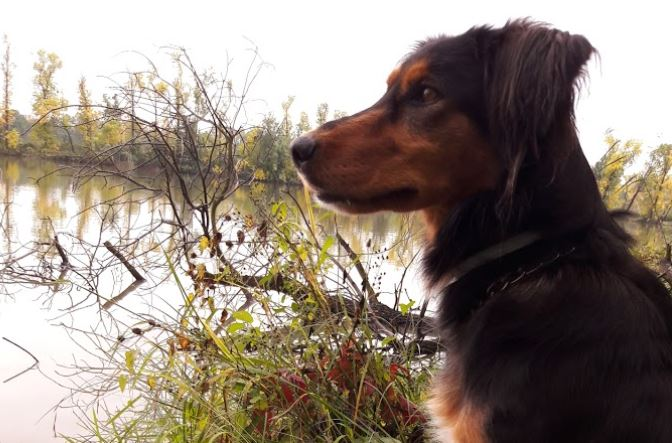
\includegraphics[width = 0.3\textwidth]{"O:/latex kurz/automate_figures/figures/daisy (24).JPG"}}
\subfloat[]{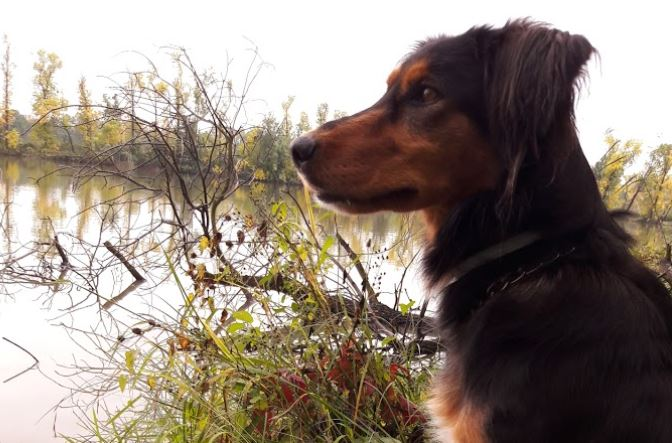
\includegraphics[width = 0.3\textwidth]{"O:/latex kurz/automate_figures/figures/daisy (25).JPG"}}\\
\subfloat[]{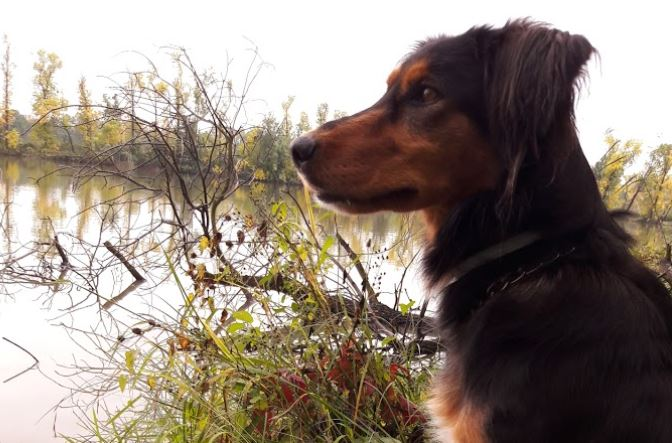
\includegraphics[width = 0.3\textwidth]{"O:/latex kurz/automate_figures/figures/daisy (26).JPG"}}
\subfloat[]{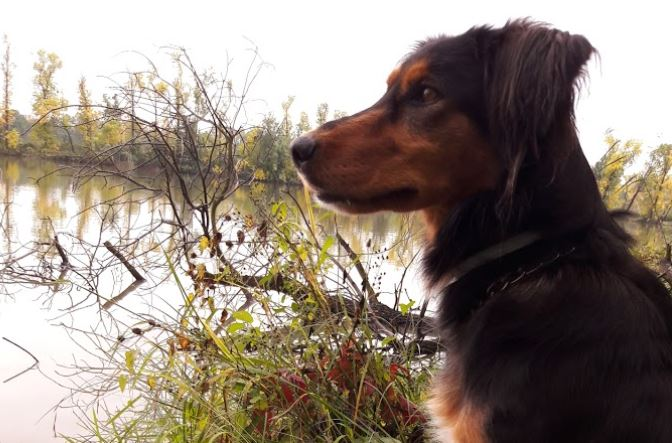
\includegraphics[width = 0.3\textwidth]{"O:/latex kurz/automate_figures/figures/daisy (27).JPG"}}
\subfloat[]{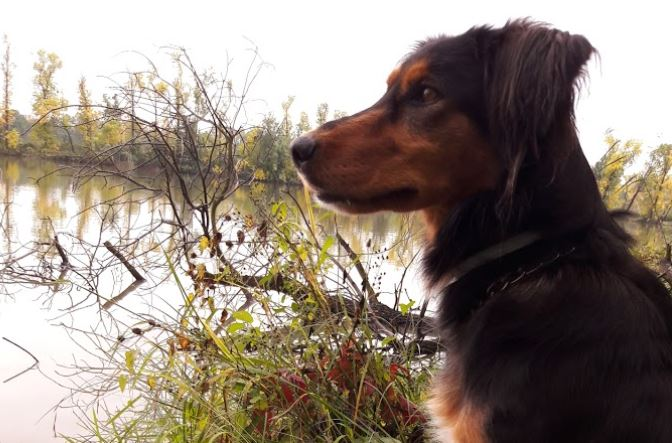
\includegraphics[width = 0.3\textwidth]{"O:/latex kurz/automate_figures/figures/daisy (28).JPG"}}\\
\subfloat[]{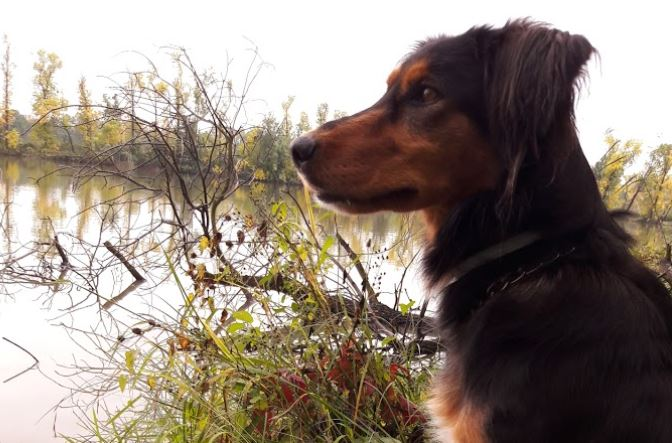
\includegraphics[width = 0.3\textwidth]{"O:/latex kurz/automate_figures/figures/daisy (29).JPG"}}
\subfloat[]{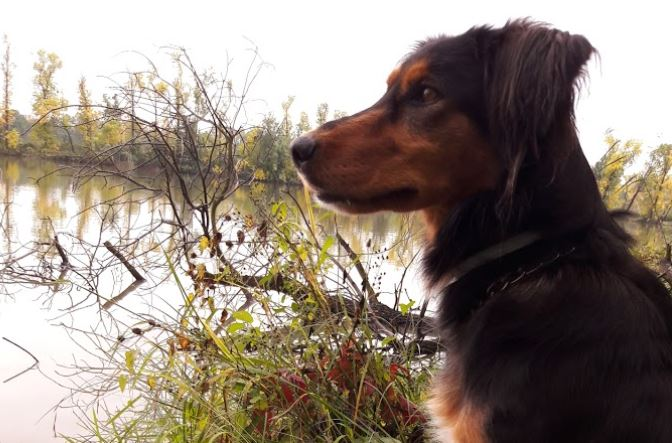
\includegraphics[width = 0.3\textwidth]{"O:/latex kurz/automate_figures/figures/daisy (3).JPG"}}
\subfloat[]{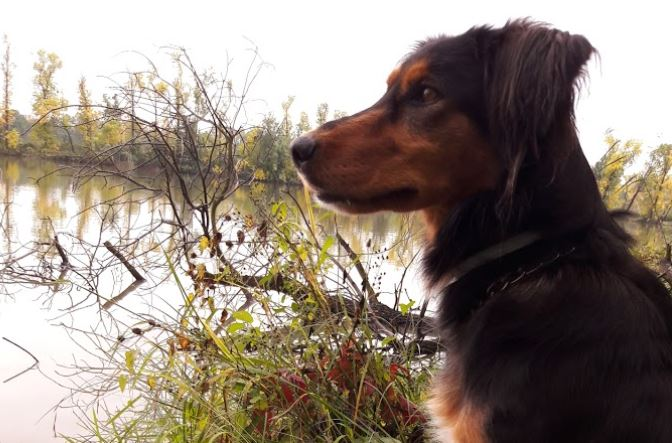
\includegraphics[width = 0.3\textwidth]{"O:/latex kurz/automate_figures/figures/daisy (30).JPG"}}\\
\caption{Caption for the figures.}
  \label{supp-fig-2}
  \end{figure}
  
  \begin{figure}

\subfloat[]{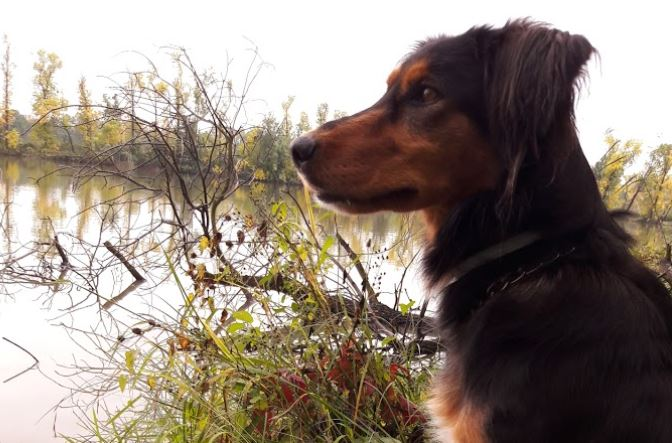
\includegraphics[width = 0.3\textwidth]{"O:/latex kurz/automate_figures/figures/daisy (4).JPG"}}
\subfloat[]{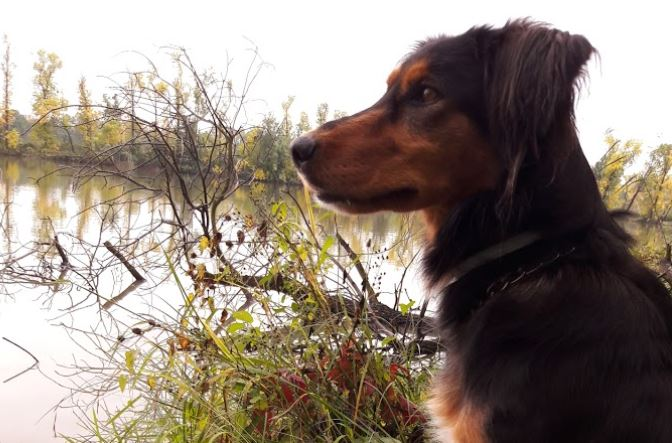
\includegraphics[width = 0.3\textwidth]{"O:/latex kurz/automate_figures/figures/daisy (5).JPG"}}
\subfloat[]{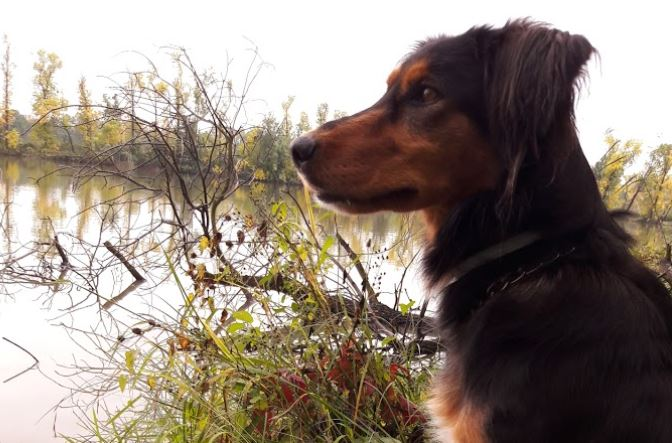
\includegraphics[width = 0.3\textwidth]{"O:/latex kurz/automate_figures/figures/daisy (6).JPG"}}\\
\subfloat[]{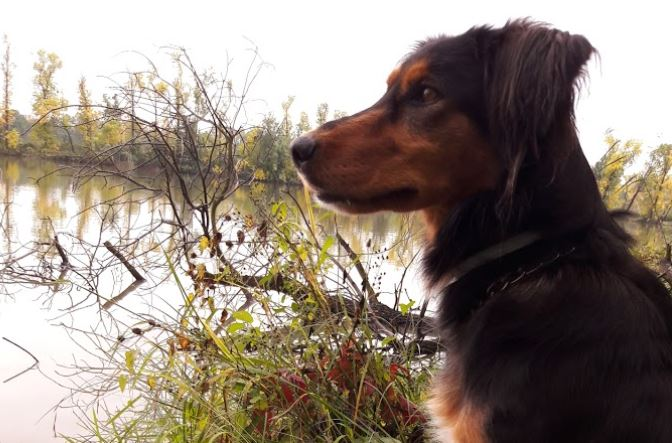
\includegraphics[width = 0.3\textwidth]{"O:/latex kurz/automate_figures/figures/daisy (7).JPG"}}
\subfloat[]{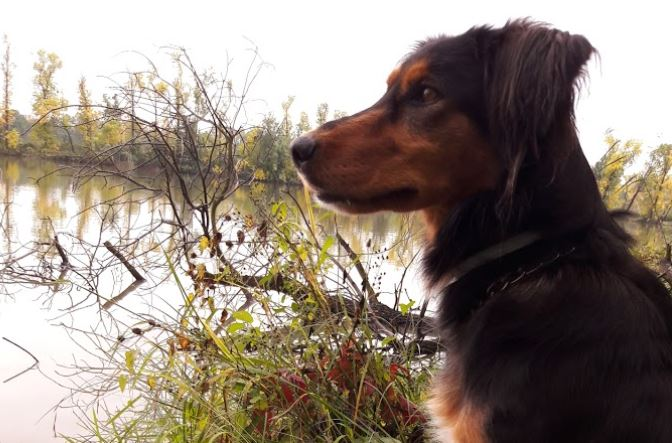
\includegraphics[width = 0.3\textwidth]{"O:/latex kurz/automate_figures/figures/daisy (8).JPG"}}
\subfloat[]{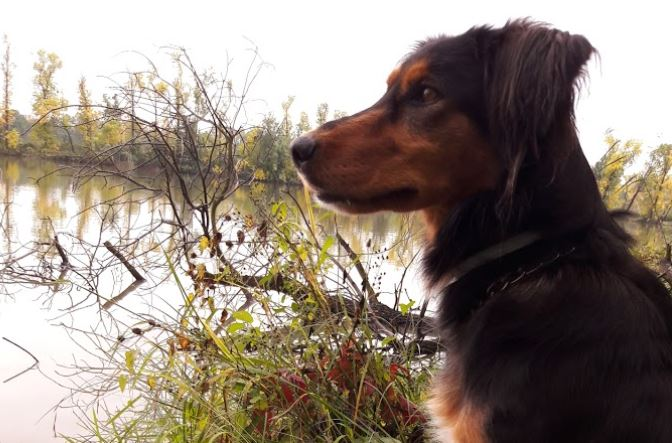
\includegraphics[width = 0.3\textwidth]{"O:/latex kurz/automate_figures/figures/daisy (9).JPG"}}\\
\caption{Caption for the figures.}
  \label{supp-fig-3}
  \end{figure}
  \end{document}
